\Chapter{RÉSULTAT EXPÉRIMENTAUX}\label{sec:Theme2}

Nous présentons les résultats en commençant par décrire l’implémentation du modèle conceptuel du robot logiciel codeur présenté dans la sous-section~\ref{subsection_cadre_conceptuel}. Ensuite, nous présenterons successivement les résultats propres à chacun des sous-objectifs décrits dans le chapitre~\ref{chapitre_methode}.

\section{Implémentation: du modèle conceptuel au modèle opérationnel}

L’implémentation de la machine (conceptuelle) est passée par la programmation manuelle d’une première interface et d’un premier noyau, en mettant à jour une version préliminaire de générateur, basée sur une GUI\cite{bluiksnot_repo} en lui intégrant la capacité de générer du code à partir d’un module externe via son \textit{hook} au moment de l’installation. La version à ce jour, ainsi que ses guides d’utilisation et ses scripts associés, sont disponibles sur le site de ERPLibre\footnote{\url{https://erplibre.ca}}.

L’interface permet l’interactivité avec un utilisateur ou le système-cible. Dans le cadre conceptuel~\ref{subsection_cadre_conceptuel}, l’interface est découplée en deux ensembles de méta-données: µ$_C^A$ et µ$_C^B$. µ$_C^B$ est l’ensemble qui paramétrise le passage de méta-données au code pour un module spécifique. µ$_C^A$ est l’ensemble qui paramétrise le passage de code aux méta-données, tout en préparant un µ$_C^B$ adapté à ce module spécifique. Ce découplage a permis l’adaptation de l’interface au contexte de l’installation de modules sur une instance Odoo via des \textit{hooks}. Par la suite, un ensemble supplémentaire de méta-données, noté µ$_C^0$, a été dégagé de la programmation manuelle de versions successives de µ$_C^A$. µ$_C^0$ sert à initialiser une version de départ de µ$_C^A$.

Le noyau prend les paramètres issus de l’interface pour créer des méta-données, générer l’ensemble des fichiers des modules désirés (mode direct) et faire de la rétro-ingénierie (mode indirect) sur des modules existants.

\subsection{Développement et amélioration continue}

Dans la Figure~\ref{fig:dia_sequence_gc}, µ$_C^0$, µ$_C^A$, µ$_C^B$, $C$ et $M$ sont tous des modules installables sur Odoo. $M^i$ et $M^d$ sont des sections de code dans le module $M$. µ$_C^0$, µ$_C^A$ et µ$_C^B$ dépendent de $M$. µ$_C^A$, ce sont les macro-méta-données, alors que µ$_C^B$, sont les micro-méta-données.

\begin{figure}
\centering
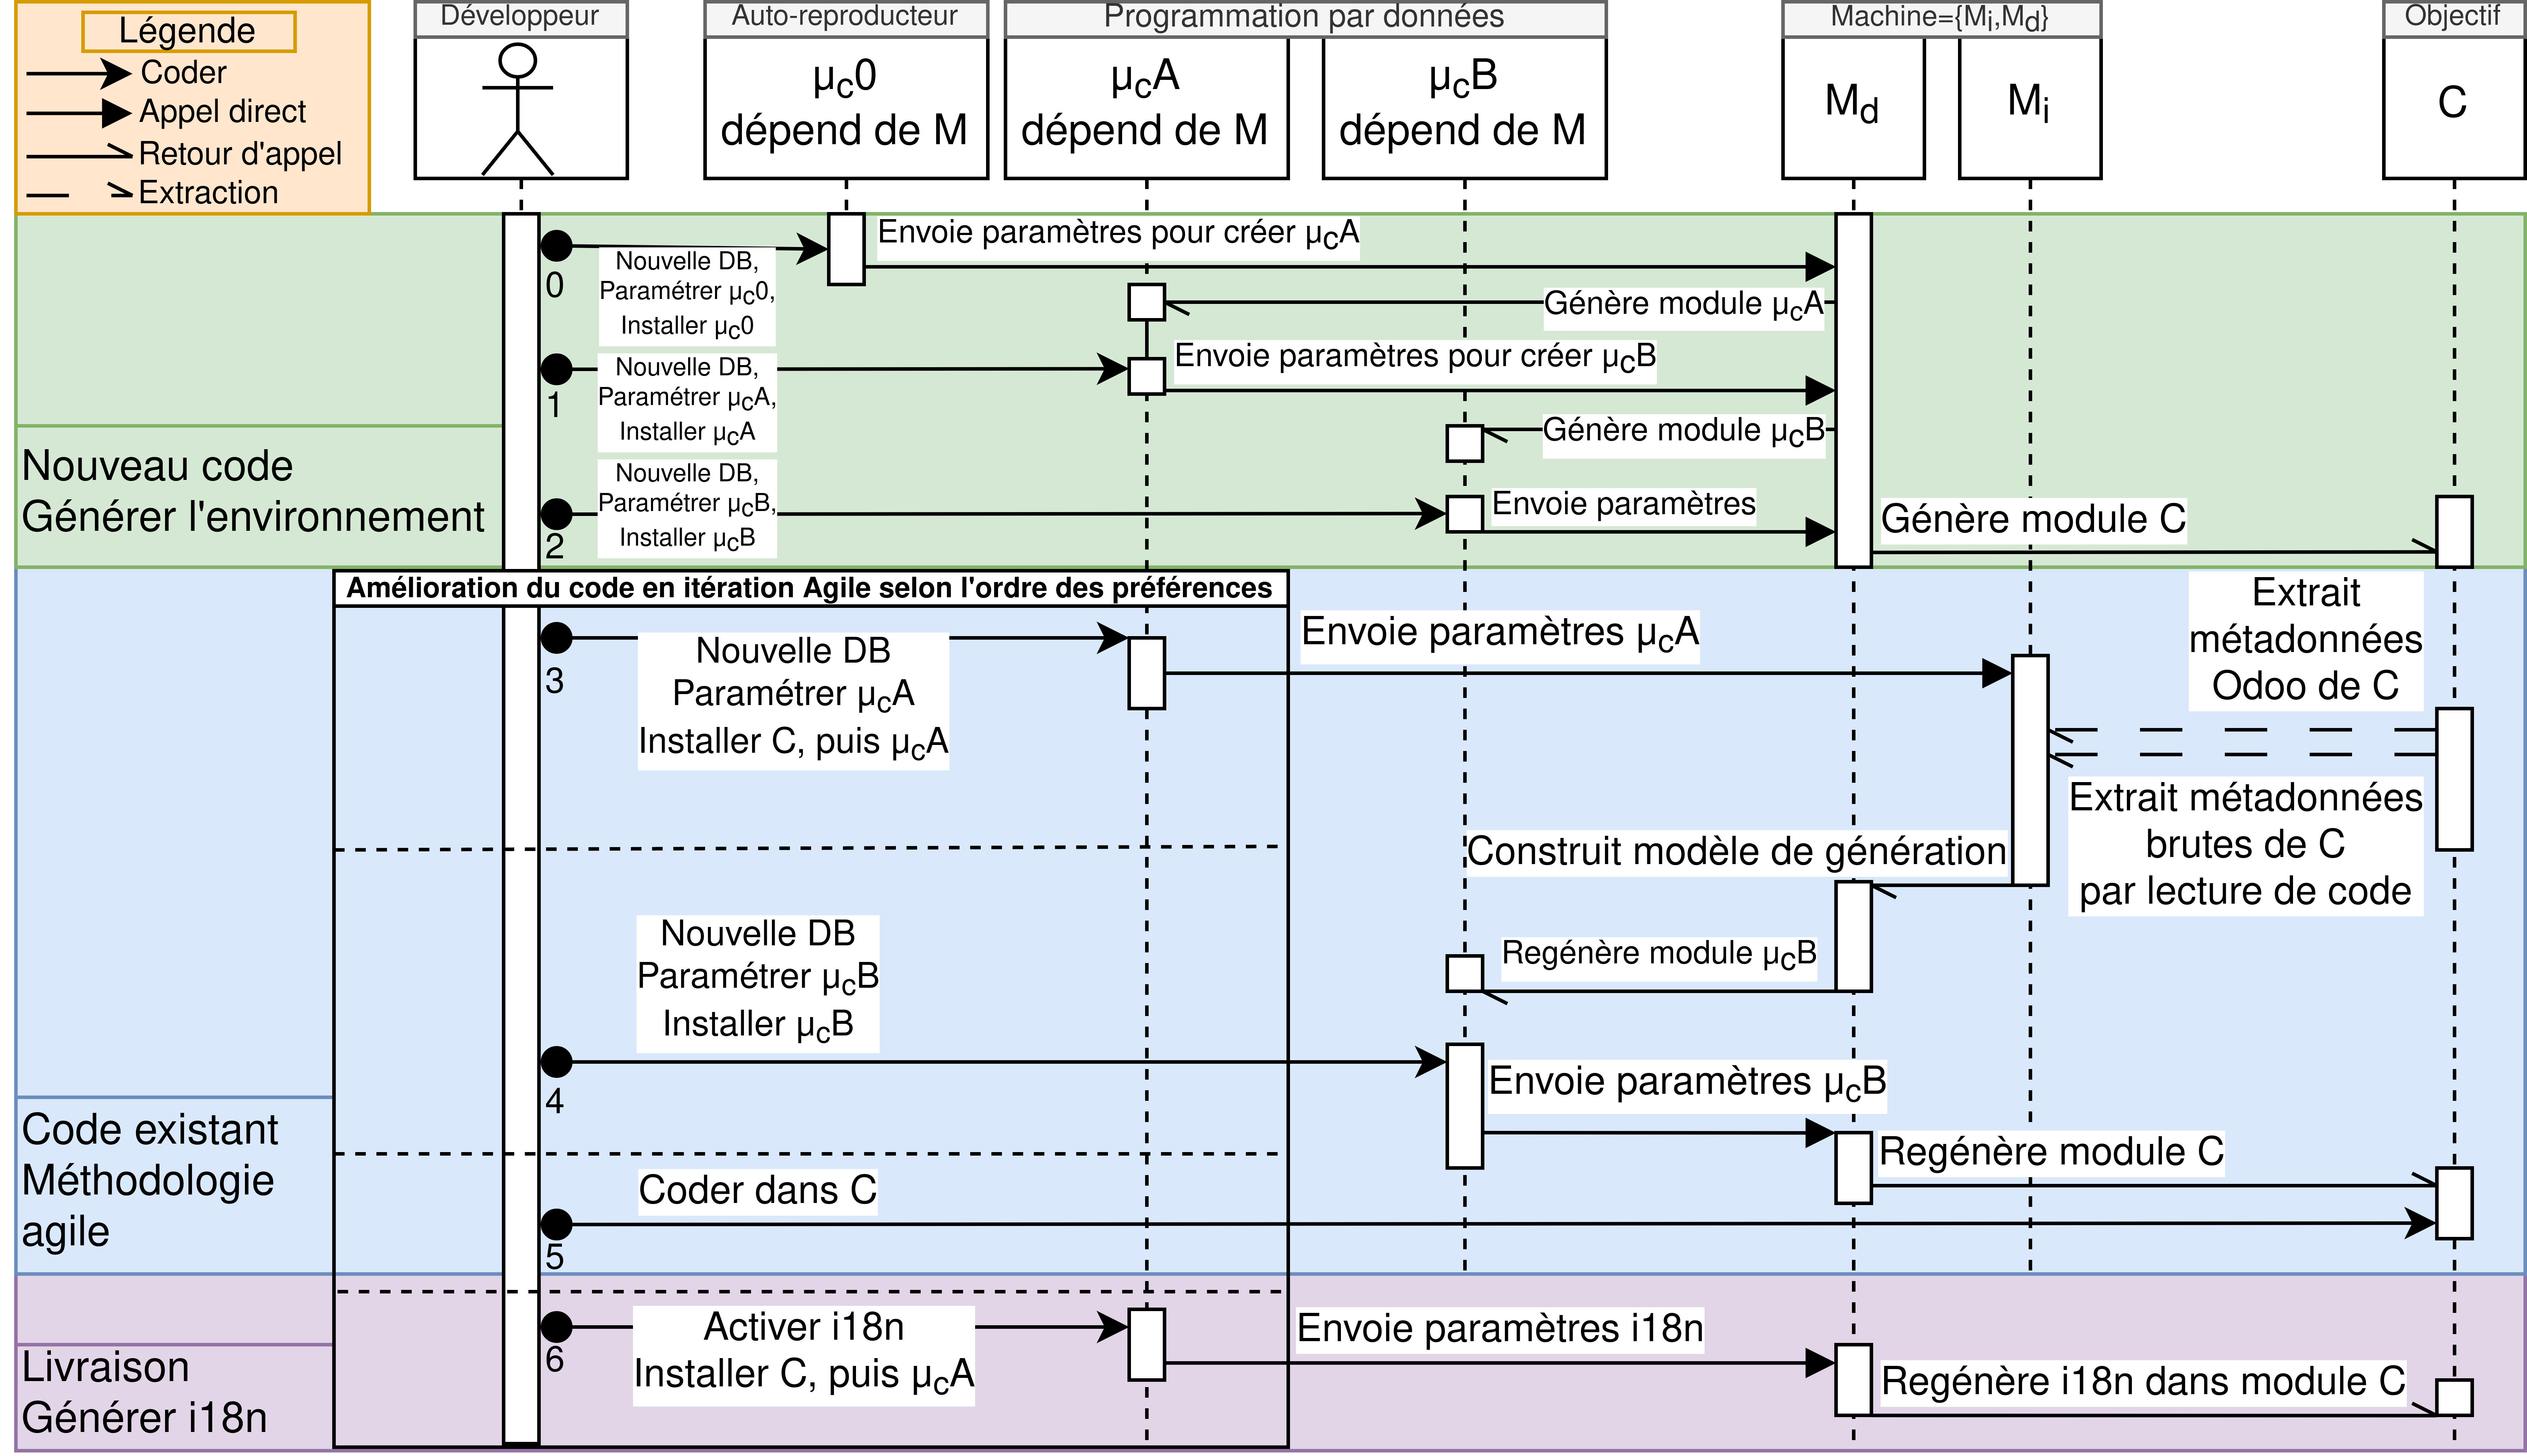
\includegraphics[width=6.535in]{images/code_generateur_erplibre_global_sequence.drawio.png}
\caption{Interaction du développeur avec le générateur de code}
\label{fig:dia_sequence_gc}
\end{figure}

Au départ d’un nouveau module code, µ$_C^0$ génère µ$_C^A$ qui génère µ$_C^B$ qui génère $C$. Il existe un script qui automatise un nouveau code, le développeur peut paramétrer le nom des modules et leurs emplacements. Ensuite, le développement commence en itérations agiles, les actions de 3 à 6 peuvent être exécutées dans l’ordre du choix du développeur.

Passer par l’étape 3 permet de mettre à jour l’étape 4, selon l’état du code, grâce à la rétro-ingénierie. L’étape 4 permet de mettre à jour le code selon le générateur. Il est possible de générer de nouvelles sections, comme la vue portail. Passer à l’étape 5 permet de personnaliser le code directement alors que l’étape 6 permet de mettre à jour le i18n de manière automatique.

La livraison sert à générer le i18n. C’est Odoo qui le génère, mais le générateur envoie les commandes, la liste des langues désirées à supporter et place les fichiers aux bons endroits dans le module. La raison pour laquelle c’est µ$_C^A$ qui doit le générer, c’est parce que le module doit être fini d’être généré et chargé de nouveau, pour ensuite générer les langues, sinon elles sont corrompus par les traces de µ$_C^B$.

% TODO mettre dans discussion : Dans un contexte où l’ingénierie et la rétro-ingénierie serait parfaite, on n’aura pas besoin de mémoriser µ$_C^A$ et µ$_C^B$. Entre-temps, il y a une intervention humaine sur chacun de ces modules pour accélérer le développement. L’outil Git est utilisé pour faire des comparaisons entre les états d’itérations, seul ce qui est commité contient le bon contenu.

\subsection{Architecture}\label{architecture_result}
La présente section décrit et explique l'architecture choisie.

La Figure~\ref{fig:dia_architecture} démontre un développeur qui utilise l'interface de la machine qui opère dans le noyau de la machine.

\begin{figure}
\centering
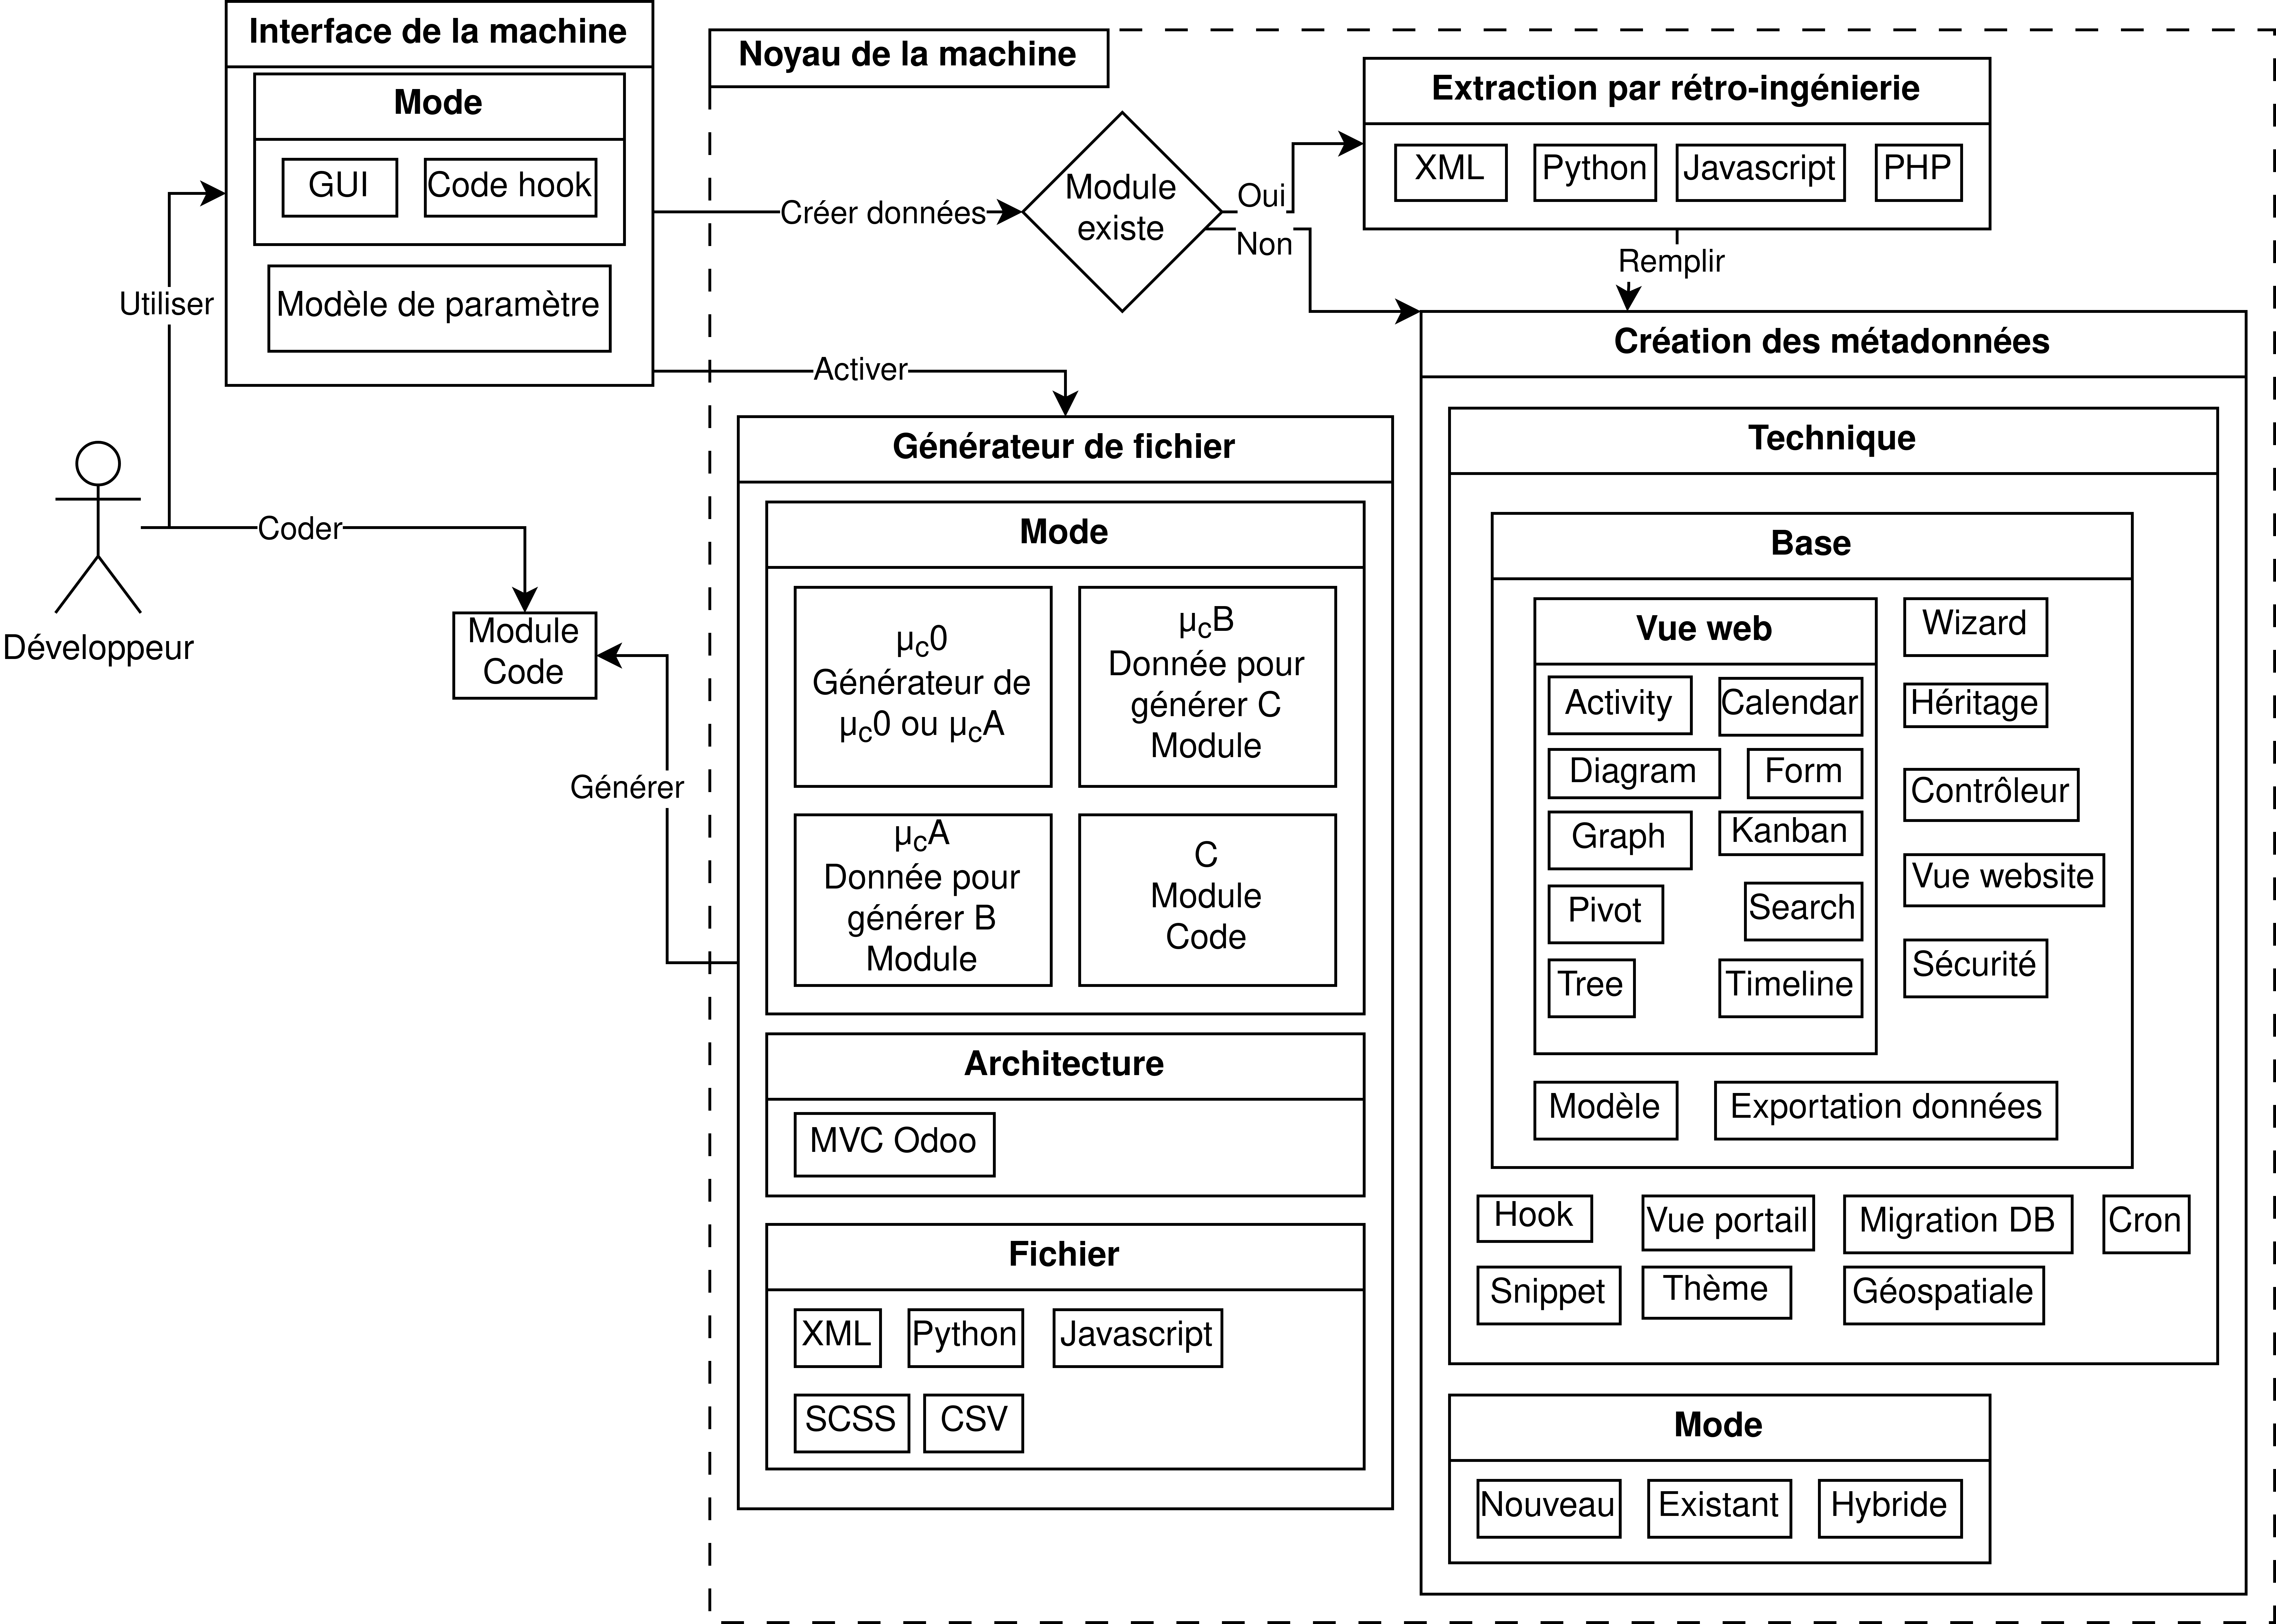
\includegraphics[width=6.535in]{images/architecture_machine.drawio.png}
\caption{Architecture du générateur de code dans son ensemble, nommé machine. Le développeur peut modifier le code source directement ou utiliser l'interface de la machine qui passe par un ensemble de composantes.}
\label{fig:dia_architecture}
\end{figure}

La section de l’interface machine permet à l’utilisateur de créer un modèle de données pour indiquer à la machine quelle opération effectuer avec les données associées. Plusieurs combinaisons, héritables, sont possibles, selon les différentes techniques. De plus, c’est ici que l’on vient activer la génération de code.

La section de l’extraction par rétro-ingénierie permet de remplir le modèle de méta-données, sans passer par la paramétrisation. Ça extrait des informations qui ne sont pas accessibles dans le modèle de données d’Odoo sur le module.

La section de la création de méta-données se fait soit par l’utilisateur via la GUI ou par le «Code \textit{Hook}», il gère simultanément plusieurs techniques qui sont dans des modules. Le mode «nouveau» permet de créer de nouvelles données. Une fois qu’elles sont créées, c’est le mode «existant» qui est utilisé. Cependant, le mode «hybride» permet d’écraser les données existantes en réactivant le mode «nouveau».

La section du générateur de fichiers se fait activer par l’interface, mais prend les méta-données pour faire sa génération, selon le mode qu’il doit générer et l’architecture qu’il connaît. Il fait des liaisons entre les modèles et les vues en référence aux noms des champs de chaque modèle de données.

Chacun de ces blocs de l’architecture est modulaire, chaque technique est héritable, pour modifier le comportement et ajouter des liaisons afin de permettre une génération de code.

La sécurité dépend du modèle, le contrôleur dépend du modèle et la vue dépend du contrôleur et du modèle.

\subsection{Auto-générateur}

On arrive à l'auto-générateur représenté par µ$_C^0$, voir Annexe~\ref{annexe_cg_code_uc0}. Au moment de l'installation de celui-ci, il génère le même code que lui-même, au même endroit dans le système de fichiers. Une légère modification va créer une autre entité qui sera une déviation dans l’objectif de démarrer une chaîne de production logicielle.

C'est le module $M$ qui contient les méta-données de µ$_C^0$. Ainsi, exécuter µ$_C^0$ devient un test de fonctionnalité et on obtient un succès lorsqu'il n'y a pas de différence. Cependant, sa programmation est actuellement spécifique à sa génération, aucun autre module n’a besoin de cette fonctionnalité unique.

L'auto-générateur est utilisé pour générer des µ$_C^A$ avec une légère modification dans les paramètres. Même s'il a la capacité de générer un µ$_C^B$, mieux vaut créer la chaîne proposée pour faire de l'amélioration continue.

\section{Résultats propres à SO-1}
Nous examinerons maintenant les résultats propres à chaque sous-objectif décrit dans le chapitre 3, méthode.

À l'intérieur de cette section, le code généré est fonctionnel et utilisable selon des techniques désirées. Cependant, ce code existe et est fonctionnel dans certaines limitations. En effet, la génération de code est peu paramétrable, elle sert de base au développeur pour qu'il personnalise ce code à ses propres contextes fonctionnels. En pratique, le développeur doit toujours faire de la réingénierie sur le code généré. L'avantage est que le développement est accéléré, puisqu'une base fonctionnelle solide est créée.

\subsection{Génération par gabarit}

La génération par gabarit était déjà supportée dans la version initiale~\cite{bluiksnot_repo}, de plus, il y a eu des améliorations telles que l'utilisation des \textit{f-strings} au lieu d'utiliser la fonction \textit{format} de \textit{String}, l'utilisation de la bibliothèque Code-writer en Python\footnote{\url{https://pypi.org/project/code-writer/}} et l'utilisation de la bibliothèque lxml\footnote{\url{https://pypi.org/project/lxml/}}.

\subsection{Génération de l'architecture MVC}

L’architecture MVC était déjà supportée dans la version initiale~\cite{bluiksnot_repo}, de plus, il y a eu des améliorations telles que les règles de sécurité sont ajustées selon les configurations et personnalisables par la suite et l'ajout de bouton qui ouvre des \textit{Wizard}\footnote{\url{https://github.com/ERPLibre/odoo-code-generator/tree/9d79f67/code_generator/wizards}} pour générer les vues, les modèles et les contrôleurs, voir Figure~\ref{fig:dia_gui_mvc}, Figure~\ref{fig:dia_wizard_mvc} et le tableau~\ref{tab:stat_code_wizard_mvc} sur les statistiques du code. Ainsi, le développeur peut les configurer et demander de générer les méta-données associées.

\begin{figure}[htb]
\centering
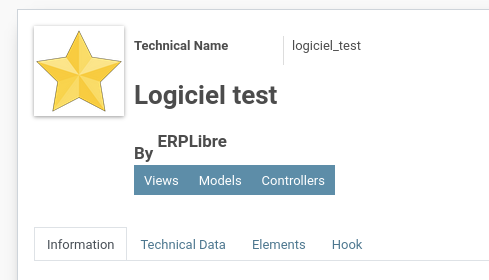
\includegraphics[width=3in]{images/GUI_MVC.png}
\caption{Exemple support MVC dans GUI du générateur de code}
\label{fig:dia_gui_mvc}
\end{figure}

\begin{figure}[htb]
\centering
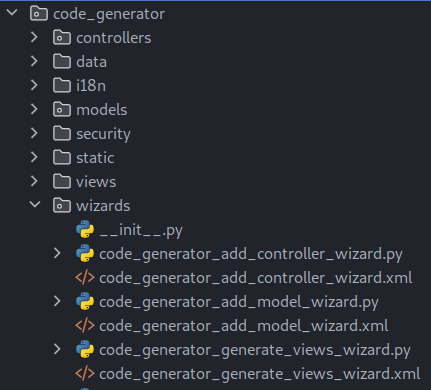
\includegraphics[width=3in]{cg_wizard_mvc.png}
\caption{Démonstration du code pour le MVC dans la section \textit{wizards} du module du générateur de code}
\label{fig:dia_wizard_mvc}
\end{figure}

\begin{table}[htb]
\caption{Statistiques sur le code des «wizards» sur la GUI qui gère la génération de MVC}
\centering
\begin{tabular}{|l|l|l|l|l|l|l|}

\hline
\cellcolor[HTML]{d9d9d9}{\textbf{Langage}} & \cellcolor[HTML]{d9d9d9}{\textbf{Fichiers}} & \cellcolor[HTML]{d9d9d9}{\textbf{\%}} & \cellcolor[HTML]{d9d9d9}{\textbf{Lignes de code}} & \cellcolor[HTML]{d9d9d9}{\textbf{\%}} & \cellcolor[HTML]{d9d9d9}{\textbf{Commentaire}} & \cellcolor[HTML]{d9d9d9}{\textbf{\%}}\\\hline

Python & 5 & 55.6 & 1809 & 58.5 & 560 & 17.3\\\hline
XML & 4 & 44.4 & 178 & 92.7 & 10 & 5.2\\\hline
\textbf{Total} & \textbf{9} & \textbf{100.0} & \textbf{2068} & \textbf{60.4} & \textbf{570} & \textbf{16.6}\\\hline

\end{tabular}
\label{tab:stat_code_wizard_mvc}
\end{table}

\subsection{Générer un module à partir d’une base de données externes}

La migration de données à partir de SQL était déjà supportée dans la version initiale~\cite{bluiksnot_repo}, cependant il y a eu des améliorations\footnote{\url{https://github.com/ERPLibre/odoo-code-generator/tree/9d79f67/code_generator_db_servers}}, telles que l'ajout de types de données, dont ceux utilisés par le projet Accorderie, l'ajout d'associations entre les types de données et les différentes personnalisations de l’architecture Odoo, la modification de l'interface qui représente la base de données avec les contrôleurs pour permettre la configuration de la migration sur le modèle de données désiré et la gestion des interdépendances entre modèles. Pour gérer le problème d'interdépendances, il a fallut créer une séquence de création des données avec une seule dépendance et, à la toute fin, ajouter l'interdépendance en mettant à jour les données. Il y a eu au moins 1639 ajouts de lignes de code, voir Figure~\ref{fig:dia_cg_db_servers}.

\begin{figure}[htb]
\centering
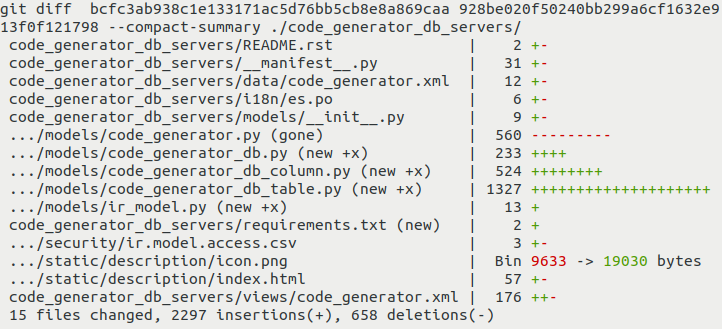
\includegraphics[width=4in]{git_diff_code_generator_db_servers.png}
\caption{Démonstration des modifications effectués pour adapter le code de la migration de base de données pour supporter plus de fonctionnalités.}
\label{fig:dia_cg_db_servers}
\end{figure}

\subsection{Génération de code par des données}

La génération de code par des données a la capacité de prendre les données via les interfaces utilisateurs telles que la GUI et le «Code \textit{hook}». Cela permet la personnalisation pour obtenir un logiciel adapté à ce que l’utilisateur est capable d’exprimer.

Le robot logiciel codeur est une machine qui, grâce à son interface «code \textit{hook}», se fait commander par deux couches de méta-données paramétrables par l’humain. Les deux couches interfèrent entre elles pour permettre l’évolution de la fonctionnalité désirée. Pour voir un exemple de génération de code par données, voir Annexe~\ref{annexe_cg_code_uc0}.

\subsection{Interprétation des résultats de SO-1}

\subsubsection{SO-1 Accomplissements}
Pour résumer l'ensemble des accomplissements du premier sous-objectif (SO-1), nous avons fait une simplification de l’écriture de technique dans le générateur de code avec l’utilisation de \textit{f-string}, de la bibliothèque \textit{Code-writer }et de la bibliothèque \textit{lxml}, nous avons fait un ajout de \textit{Wizard} pour configurer le MVC selon des paramètres, nous avons améliorer l’importation des bases de données externes, supporté la génération de code par des données et augmenté le nombre de techniques de génération de code, le support des \textit{templates} \textit{Qweb} et fait l'ajout du type de données géospatiales.

\subsubsection{SO-1 Feuille de route}
La brève feuille de route du premier sous-objectif se résume à implémenter les fonctionnalités manquantes dans la GUI pour générer les MVC d’un module, à augmenter le nombre de technologies à supporter sur l'importation des données, à ajouter le support de génération sur différentes architectures, à supporter différentes techniques de sécurités personnalisables, comme l’anonymisation des données, à générer automatiquement une documentation sur l’utilisation d’une technique et à supporter la génération sur d’autres systèmes \textit{ERP} libres tel que Tryton\footnote{\url{https://www.tryton.org}}

\section{Résultats propres à SO-2}

\subsection {Extraction de code et reproduction}

De la macro et micro extraction ont été réalisées avec plusieurs techniques combinées. Pour pouvoir faire de la reproduction, il a suffit de faire de la macro extraction, c'est-à-dire faire une recherche dans toutes les classes pour copier le contenu de chaque méthode pour le transformer en méta-données et pouvoir faire l’opération directe de générer le code qui a été copié. L’utilisation de l’\textit{AST} a servi à déterminer quelle ligne de code était à découper pour la recopier.

Cependant, il était nécessaire, dans certains contextes, de faire de la micro extraction, telles que l’extraction des noms des constantes, qui sont transformées en valeurs, lors de l’exécution, l’extraction des commentaires qui n’est pas supportée dans la bibliothèque \textit{AST} de Python 3.7, l’extraction des décorateurs et l’extraction des paramètres sur les méthodes.

De plus, les vues ont été extraites dans le but d'obtenir des méta-données spécifiques qui caractérisent la reconstruction de la vue, ces données n’étaient pas accessibles dans les données d'Odoo.

Tout le code en lien avec l'extraction de données se retrouve dans les fichiers\footnote{\url{https://github.com/ERPLibre/odoo-code-generator/tree/9d79f67/code_generator}} extrator\_controller.py, extractor\_module.py, extrator\_module\_file.py et extractor\_view.py, voir le tableau~\ref{tab:stat_code_extractor} pour comprendre les statistiques sur le code.

\begin{table}[htb]
\caption{Statistiques sur le code de l'extraction de données de modules Odoo}
\centering
\begin{tabular}{|l|l|l|l|l|l|l|}

\hline
\cellcolor[HTML]{d9d9d9}{\textbf{Langage}} & \cellcolor[HTML]{d9d9d9}{\textbf{Fichiers}} & \cellcolor[HTML]{d9d9d9}{\textbf{\%}} & \cellcolor[HTML]{d9d9d9}{\textbf{Lignes de code}} & \cellcolor[HTML]{d9d9d9}{\textbf{\%}} & \cellcolor[HTML]{d9d9d9}{\textbf{Commentaire}} & \cellcolor[HTML]{d9d9d9}{\textbf{\%}}\\\hline

Python & 4 & 100.0 & 1415 & 72.6 & 127 & 6.5\\\hline

\end{tabular}
\label{tab:stat_code_extractor}
\end{table}

Certaines informations ont été extraites dans le \textit{Javascript} à l’aide de la bibliothèque \textit{pyjsparser}. Pour l’extraction d'un projet externe d'une autre technologie, un extracteur de PHP a été développé via un \textit{parser} de la communauté\footnote{\url{https://github.com/JameelNabbo/PHP-Parsers}}.

% TODO manque info sur le générateur de générateur de code
C'est en développant les techniques de génération de code que nous réalisons la reproduction. Un script a été développé pour accélérer l’écriture du générateur de code, ainsi qu'un générateur de générateur de code. Ensuite, le développeur peut le transformer légèrement pour prendre les paramètres des méta-données.

\subsection {Amélioration continue sur la génération}

Grâce à l’extraction des méta-données, dès que la technique de génération est bien développée avec les méta-données, le code est automatiquement généré avec de bonnes pratiques logicielles, corrigeant automatiquement les problèmes.

L’intérêt d'utiliser Odoo pour lire le module est qu'il valide déjà certains fonctionnements. Par exemple, il n'y pas d’erreur de syntaxe dans le Python où les XML étaient bien construits.

Ainsi, pour un module désiré, nous utilisons les outils pour générer µ$_C^A$ et µ$_C^B$, puis en avançant dans le développement, nous bouclons entre le 3 et 4 sur Figure~\ref{fig:dia_sequence_gc}.

\subsection {Test de validation de génération de codes}\label{test_validation_generation_code_resultat}

Pour tester ce générateur de code, la technique du test de comparaison des sorties de la génération a été utilisée. Pour procéder, un développeur valide via l'outil Git ce qui est \textit{commité}\footnote{Un terme dans l'outil Git pour valider le code en créant un état dans l'historique.}. Ainsi, un script a été développé pour lancer en parallèle les tests et valider les différences de génération avec ce qui a été \textit{commité} précédemment. Un succès est lorsqu'il y a aucune différence dans le code entre la version générée et la précédente. Ainsi, les tests implémentés permettent de valider l’installation du module généré, de valider que µ$_C^B$ génère bien le module cible sans différence dans le code, de valider que µ$_C^A$ génère µ$_C^B$ sans différence dans le code, ainsi que valider que la migration d’une base de données SQL se fait sans différence dans le code.

En exécutant tous les tests, voir Annexe~\ref{annexe_test_generateur_code}, une couverture de 84\% est obtenue, tous les tests présents sont un succès, sauf ceux sur l’auto-générateur.

Les tests deviennent une documentation sur l'utilisation du générateur de code. Puisque la génération de code se fait par données, il suffit de changer les paramètres pour générer un autre module et lancer un nouveau projet sur le module généré pour obtenir toute la chaîne.

\subsection {Règles de codage standardisées}

Au moment de générer les fichiers, toutes les sorties textes sont traitées par des outils de mise en forme, en suivant des règles de codage standardisées.

Pour le Python, l’outil \textit{black} est utilisé pour la mise en forme en suivant le standard PEP8 avec \textit{isort} pour réordonner les importations. \textit{Black} donne une mise en forme non naturelle comparée à l’écriture de code pour un humain. Cependant, son résultat facilite la lecture et le suivi des différences pour les futurs ajouts. Le Javascript, le HTML et le XML sont mis en forme avec l’outil Prettier.

De plus, le générateur force le déplacement des classes dans leur fichier respectif pour créer une classe par fichier. Les champs, pour chaque modèle, sont déplacés en ordre alphabétique, mais le premier est celui qui est utilisé pour représenter le modèle\footnote{Référence à l'attribut «\_rec\_name»}.

\subsection{Interprétation des résultats de SO-2}

\subsubsection{SO-2 Accomplissements}
Pour résumer l'ensemble des accomplissements du deuxième sous-objectif, nous avons fait de l'extraction du code via l’utilisation d’un AST et extraction des méta-données dans les fichiers XML, de l'amélioration continue sur la génération de code, grâce à la reproduction à l’aide de l’extraction du code, développé un outil pour aider à la création de technique de génération à l’aide d’un générateur de générateur de code, intégré dans le générateur de code des tests de validation en reproduisant l’ensemble des techniques en démonstration, ainsi qu'appliquer des règles de codage standardisées sur la génération de code.

\subsubsection{SO-2 Feuille de route}
La brève feuille de route du second sous-objectif se résume à finaliser l’implémentation de l'auto-génération sur le générateur de code, de mettre à jour les tests pour atteindre une couverture de code à 100\% et d'ajouter des tests sur les techniques d’extractions de code tel que le PHP.

\section{Résultats propres à SO-3}

\subsection{Classification des techniques développées}\label{result_technique_developpe}

En référence à la Figure~\ref{fig:dia_architecture}, les techniques «Modèle», «\textit{Form}», «\textit{Tree}», «Contrôleur» et «Migration \textit{DB}~\footnote{Module de migration de base de données}», étaient déjà implémentées dans la version initiale~\cite{bluiksnot_repo}, mais elles ont reçu des améliorations pour s’agencer aux autres techniques. Les autres techniques ont été développées pour permettre une modularité aux modules à générer, puis supporter de nouvelles fonctionnalités telles que la gestion des cartes interactives avec le géospatial.

% TODO faire un diagramme des dépendances
% Les techniques :
% \begin{enumerate}
%     \item Contrôleur;
%     \item Cron;
%     \item Exportation des données;
%     \item Géospatiale (dépend de Modèle);
%     \item Héritage;
%     \item Hook;
%     \item Migration DB\footnote{importation des données par DB};
%     \item Modèle;
%     \item Portal;
%     \item Sécurité;
%     \item Snippet;
%     \item Thème;
%     \item Vue web;
%     \begin{enumerate}
%         \item Activity;
%         \item Calendar;
%         \item Diagram;
%         \item Form;
%         \item Graph;
%         \item Kanban;
%         \item Pivot;
%         \item Search;
%         \item Timeline;
%         \item Tree;
%     \end{enumerate}
%     \item «website\_leaflet» (dépend de Snippet et Géospatiale);
%     \item Wizard;
% \end{enumerate}

\subsection{Interface du générateur de code}

\subsubsection{L'interface graphique}

 L'interface graphique existait déjà dans la version initiale~\cite{bluiksnot_repo}, elle a été améliorée pour afficher plus d'informations par rapport au développement. Elle sert à faciliter la paramétrisation du générateur de code. Elle n’a pas été priorisée et elle manque de fonctionnalités si nous la comparons à ce qui peut être supporté via la technique \textit{code hooks} avec µ$_C^A$ et µ$_C^B$. L'interface permet de créer un module, de renommer un module, d'ajouter des modèles, voir Annexe~\ref{annexe_cg_gui_model}, et des champs, voir Annexe~\ref{annexe_cg_gui_champs}, d'ajouter des menus, d'ajouter de la sécurité, de changer les icônes, de changer les informations sur les propriétés \textit{manifest }du module, d'ajouter du code, voir Annexe~\ref{annexe_cg_gui_code} et de modification des \textit{hooks}, voir Annexe~\ref{annexe_cg_gui_hook};

\subsubsection{L'interface \textit{code \textit{hook}}}

L'interface \textit{code \textit{hook}}, voir exemple à l'Annexe~\ref{annexe_cg_code_uc0}, permet d’accéder à la totalité des fonctionnalités du générateur de code via µ$_C^A$ et µ$_C^B$. Elle a été utilisée pour toutes les démonstrations qui servent de tests et elle contient la paramétrisation pour les modules désirés. De plus, l'avantage de cette interface est qu'elle nous permet d'ajouter du code pour rendre dynamique la paramétrisation.

\subsection{Interprétation des résultats de SO-3}

\subsubsection{SO-3 Accomplissements}
Pour résumer l'ensemble des accomplissements du troisième sous-objectif, nous avons fait l'ajout de nouvelles techniques et une classification de celles-ci, nous avons rendu accessible une interface graphique pour paramétrer la génération de code et avons rendu accessible une interface de programmation pour utiliser toutes les fonctionnalités du robot logiciel codeur.

\subsubsection{SO-3 Feuille de route}
La brève feuille de route du troisième sous-objetif se résume à ajouter des paramètres pour faire davantage de personnalisation sur les techniques, à extraire les techniques du générateur et les implémenter une par module, à supporter les fonctionnalités manquantes sur toutes les techniques pour l’interface graphique et à supporter l’accès à la création de méta-données par la rétro-ingénierie via l’interface graphique.

\section{Résultats propres à SO-4}

\subsection{Utilisation d’un conteneur Docker}

Puisque le générateur de code fait partie de ERPLibre, la version 1.5.0 contient les modules de génération de code. Le déploiement se fait rapidement en utilisant le logiciel Docker et le générateur de code permet l’utilisation de l’interface graphique pour générer des modules Odoo.

\subsubsection{SO-4 Feuille de route}
La brève feuille de route du quatrième sous-objectif se résume à développer une synchronisation entre les instances pour permettre la redondance, à développer une gestion de son infrastructure via le générateur de code, à faire participer le robot logiciel codeur à la maintenance de l’infrastructure de déploiement, à utiliser d’autres systèmes de conteneur en distribution qui sont libres comme «\textit{Pod}»~\footnote{\url{https://podman.io/}} et à développer la capacité du robot logiciel codeur de valider techniquement si le logiciel est AGPLv3 au moment de l’exécution.

\section{Résultats propres à SO-5}
Le cinquième sous-objectif met en relation le générateur de code avec la communauté. Le but du générateur de code n'est pas de remplacer les humains, mais de mieux les outiller et soutenir la communauté. De plus, le cinquième sous-objectif présente les deux cas d'étude propres à ce mémoire.
\subsection{Guide : créer une communauté autour d’une technologie pour un réseau d’entraide libre}

% Un guide hybride a été produit pour comprendre les aspects cités du démarrage d’un projet, de gestion d’une communauté autour d’un projet libre et des règles d'hébergement libres. 

Avant de démarrer un projet, nous suggérons au gestionnaire de projet de suivre le guide en 7 étapes, voir Annexe~\ref{annexe_demarrer_projet_7_etape}, qui permet de démarrer rapidement un projet et de s'assurer que les membres impliqués du réseau d'entraide comprennent les mêmes enjeux et s'alignent dans la même direction. Par la suite, nous proposons le guide suivant pour gérer l'intégration d'un membre en communauté, voir Annexe~\ref{annexe_guide_integration_membre}. De plus, nous encourageons les bonnes habitudes en communauté avec le guide suivant pour la gestion du comportement en communauté, voir Annexe~\ref{annexe_guide_comportement}. Ensuite, pour se préparer au développement public, nous conseillons le guide suivant, voir Annexe~\ref{annexe_guide_dev_public}. Les problèmes peuvent survenir entre les membres de la communauté, c'est pourquoi nous suggérons le guide suivant pour faciliter la résolution de problème, voir Annexe~\ref{annexe_guide_resolution_probleme}. La communauté a besoin ensuite de formation technique et fonctionnelle, voir Annexe~\ref{annexe_guide_documentation}. Puis la sécurité est importante pour protéger les données dans la communauté, ce pourquoi nous suggérons les étapes suivantes à intégrer au projet communautaire, voir Annexe~\ref{annexe_guide_securite}. Finalement, en lien avec le développement libre, nous suggérons les étapes suivantes, voir Annexe~\ref{annexe_guide_libre}.

% \section{Projets divers}

\subsection{Projet module «auto\_backup»}

Le module «auto\_backup»\footnote{\url{https://github.com/ERPLibre/server-tools/tree/f6054fc/auto_backup}} est le premier module de la communauté de l'organisation OCA répertoire \textit{server-tools} à avoir été testé dans ce projet, un µ$_C^A$\footnote{\url{https://github.com/ERPLibre/odoo-code-generator-template/tree/b5ae8e/code_generator_template_demo_sysadmin_cron}} et µ$_C^B$\footnote{\url{https://github.com/ERPLibre/odoo-code-generator-template/tree/b5ae8e/code_generator_auto_backup}} ont été générés. Le générateur de code a pu modifier le module pour appliquer de la qualité logicielle qui a permis de développer la technique de gestion des \textit{cron}, en lançant des sauvegardes, par SSH ou en local, à des moments spécifiques dans le temps.

% \subsection{Projet module \textit{workflow} \textit{design}}

% C’est un module de gestion de projet qui a été développé entièrement avec le générateur de code qui permet de faire le suivi sur les opportunités, les menaces, les forces, les faiblesses et les objectifs. Il a été utilisé dans le projet Accorderie.

% \subsection{Projet module STARS}

% Le module STARS dépend de l’application Projet, il permet de configurer une procédure intégrée dans un projet pour suivre les étapes de STARS, voir Figure~\ref{fig:workflow_stars}.

% \begin{figure}
% \centering
% 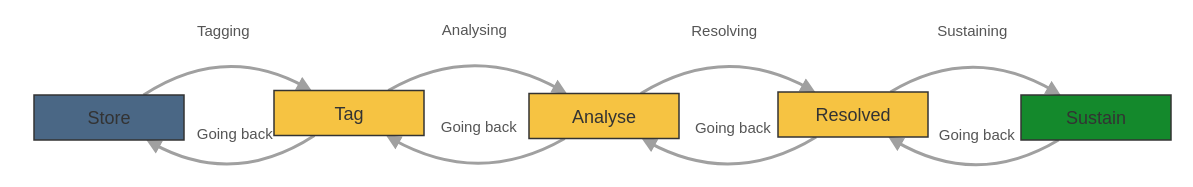
\includegraphics[width=6.535in]{workflow_stars.png}
% \caption{Procédure STARS dans l'application Projet vue Diagramme}
% \label{fig:workflow_stars}
% \end{figure}

% Ainsi, nous pouvons créer un nouveau projet et suivre cette procédure en ajoutant des tâches d'amélioration continue de son organisation, voir Figure~\ref{fig:kanban_stars}.

% \begin{figure}
% \centering
% 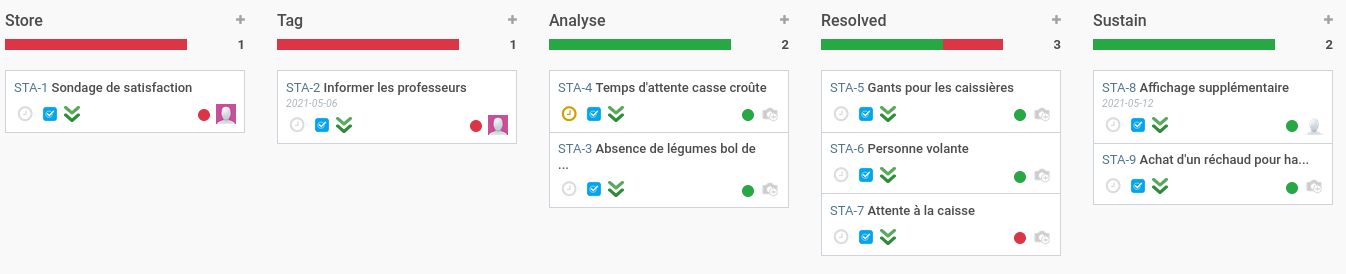
\includegraphics[width=6.535in]{kanban_stars.png}
% \caption{Suivi des tâches de projet avec procédure STARS en vue Kanban}
% \label{fig:kanban_stars}
% \end{figure}

\subsection{Projet module SRS}

Le module de spécification des exigences logiciels (SRS), c’est un module de gestion de projet qui a été développé entièrement avec le générateur de code\footnote{\url{https://github.com/ERPLibre/scrummer/tree/45ef25/code_generator_project_srs}}\footnote{\url{https://github.com/ERPLibre/scrummer/tree/45ef25/code_generator_template_project_srs}}\footnote{\url{https://github.com/ERPLibre/scrummer/tree/45ef25/project_srs}}. Il permet de faire l’analyse des besoins pour ensuite passer à l’analyse fonctionnelle et, finalement, définir les requis fonctionnels d’un projet. Il a été utilisé, entre autres, pour le projet Accorderie et le projet Portail CEPPP.

\subsection{Projet espace Accorderie}

Le projet\footnote{\url{https://github.com/TechnoLibre/odoo_accorderie/tree/ae5b4c}} a débuté par l'élaboration d'une analyse des besoins fonctionnels, puis un ensemble de requis logiciels ont été rédigés avec un membre du Réseau de l'Accorderie.

Le générateur de code a permis de créer un module Odoo 12.0 avec les modèles de données de l'Accorderie calqués sur leur base de données en SQL de MariadB, voir Annexe~\ref{annexe_db_accorderie_2019}.

Plusieurs corrections ont été effectuées avant la migration : correction des noms des champs pour les uniformiser; correction des types de champs (exemple le «\textit{True}» était exprimé par la valeur «-1» dans un type «\textit{int}», ainsi ce type a été transformé en booléen); enlever les doubles dépendances par changement de l’architecture; correction des données erronées (un champs est requis, mais il manque des données pour certaines entrées). De plus, le modèle de données n’a pas été conçu pour de l’automatisation, mais plutôt pour que les échanges de services soient validés par des membres de la communauté.

Dans l'Annexe~\ref{annexe_db_accorderie_2023}, on peut observer les adaptations des champs. Par exemple, avec la table «accorderie\_echange\_service», il y a l'ajout des champs : «nb\_heure\_estime» pour avoir une prévision des heures à effectuer, «nb\_heure\_dure\_trajet» pour reconnaître le temps de déplacement, «distance\_trajet» pour connaître la distance qui sera calculée avec le projet libre \textit{Open Source Routing Machine} (OSRM).

La migration du modèle de données a été faite dans un module qui dépend de la technique \textit{Migration DB }qui permet d'importer le modèle. Certaines données nécessitent la création d’un fichier de données XML. Pour les autres données, un autre module a été créé pour ajouter les données directement dans une base de données qui sera migrée vers une mise en production.

Un portail a été généré, pour remplacer les formulaires utilisés par l'ancienne plateforme PHP pour visualiser les entrées. Cependant, cette fonctionnalité a été abandonnée, puisque cette technologie ne plaisait pas.

Une maquette a été conçue pour un nouvel espace membre. Ainsi, nous avons utilisé la technique \textit{website\_snippet} pour afficher des données sur le site web et créer des formulaires. Cette base a permis d’accélérer la création de code de communication entre le client et le serveur. À force de faire l’intégration et la personnalisation de cette maquette, il n’y a plus vraiment de code qui provient du générateur de code.

Le générateur de code a permis d’aider à créer un diagramme pour afficher le processus d’échange de temps, voir Annexe~\ref{annexe_processus_accorderie_2023}, puis une application en Javascript avec AngularJS a été développée pour afficher ce processus à l’utilisateur, une machine à état, qui permet de revenir, selon des paramètres, à un état du processus.

Dues à des limitations humaines et de temps, tout le reste du projet a dû être fait manuellement, puisque la technologie a été changée pour faciliter le développement de l’interface.

Les statistiques du travail sont démontrées dans le tableau~\ref{tab:stat_code_accorderie}.


\begin{table}[htb]
\caption{Statistiques sur l'ensemble des modules Odoo pour le projet Accorderie.}
\centering
\begin{tabular}{|l|l|l|l|l|l|l|}

\hline
\cellcolor[HTML]{d9d9d9}{\textbf{Langage}} & \cellcolor[HTML]{d9d9d9}{\textbf{Fichiers}} & \cellcolor[HTML]{d9d9d9}{\textbf{Lignes de code}}\\\hline

XML & 79 & 34711\\\hline
Python & 91 & 19434\\\hline
Javascript & 14 & 3755\\\hline
Css & 37 & 2488\\\hline
Autre & 3 & 57\\\hline
\textbf{Total} & \textbf{224} & \textbf{60445}\\\hline

\end{tabular}
\label{tab:stat_code_accorderie}
\end{table}

\subsection{Projet Portail CEPPP}

Dans le second cas d'étude pour le Projet Portail CEPPP, l'objectif était de faire une section portail pour les patients et une section administrative pour les recruteurs, les partenaires et les administrateurs de la plateforme, de rendre accessible des formulaires et d'anonymiser les données. Le mandat était de migrer les fonctionnalités de la plateforme qui a été développée sur SuiteCRM en PHP.

Un module d'extraction de PHP a été développé, mais il n'est pas accessible dans les techniques du générateur de code. Le modèle de données était directement dans le code et, puisqu'il est dynamique, il n'est pas dans la base de données. La base de données n'a pas été extraite, les données ont été exportées en \textit{Comma-separated values} (CSV) et un module d'importation des données a été développé. Au total, il y a eu 23 fichiers analysés et 2851 données extraites.

Voici les statistiques du Tableau~\ref{tab:stat_code_portail_ceppp} du code après réingénierie et adaptation des fonctionnalités à livraison de la plateforme en début septembre 2023\footnote{\url{https://portailppp.ca}}.

\begin{table}[htb]
\caption{L'évolution entre la génération et la réingénierie des statistiques sur les langages du portail CEPPP}
\centering
\begin{tabular}{|l|l|l|l|}

\hline
\cellcolor[HTML]{d9d9d9}{\textbf{Langage}} & \cellcolor[HTML]{d9d9d9}{\textbf{\# Ligne extrait}} & \cellcolor[HTML]{d9d9d9}{\textbf{\# Ligne personnalisée}} & \cellcolor[HTML]{d9d9d9}{\textbf{\# Diff}}\\\hline

XML & 6 861 & 3 856 & - 3 005\\\hline
Python & 567 & 1 564 & + 997\\\hline
Javascript & 0 & 68 & + 68\\\hline
CSV & 25 & 51 & + 26\\\hline

\end{tabular}
\label{tab:stat_code_portail_ceppp}
\end{table}

L'anonymisation n'est pas supportée par le générateur de code, puis la personnalisation enlève beaucoup de champs mis de manière générique dans les fichiers XML. 

Le modèle de données du portail CEPPP dans Odoo 12 contient 24 modèles Annexe~\ref{annexe_db_ceppp_2022}. L'interface administrateur Annexe~\ref{annexe_form_ceppp_2022} contient la fiche du patient dont les partenaires ont accès seulement qu'à la partie anonymisée Annexe~\ref{annexe_form_anonyme_ceppp_2022}.

Le nombre de lignes de XML a diminué car le générateur de code génère, de base, toutes les vues de tous les champs. Au moment de la réingénierie, il y a eu beaucoup de nettoyage et de données XML effacées. Cependant, le développeur va mettre plus de code Python pour développer des logiques qui ne sont pas supportées par le robot logiciel codeur. Le Javascript ajouté sert à supporter les dates dans le portail. L’ajout de CSV permet l’ajout de permissions et rôles pour l’anonymisation.

\subsection{Interprétation des résultats de SO-5}

\subsubsection{SO-5 Accomplissements}
Pour résumer l'ensemble des accomplissements du cinquième sous-objectif, nous avons fait un test de la génération sur un module existant de la communauté nommé «auto\_backup», des modules de gestion de projet ont été générés pour faire le suivi de la conception fonctionnelle et de l’amélioration continue, le projet Accorderie a bénéficié du générateur de code pour la migration de la base de données vers Odoo et le projet Portail CEPPP a bénéficié du générateur de code pour la migration du code PHP vers Odoo, ainsi que de l’aide au développement de la section Portail.

\subsubsection{SO-5 Feuille de route}
La brève feuille de route du cinquième sous-objectif se résume à supporter la demande de \textit{\textit{Pull Request}} sur les projets Git respectifs, lorsqu’il y a une amélioration. Il doit y avoir un suivi et valider les règles de contribution de la communauté, développer d’autres modules de gestion de projet pour l’accompagnement dans le développement de projet client, développer des modules de gestion de communauté sur des projets de logiciels libres et créer le suivi du développement des modules communautaires avec une traçabilité sur les résultats avec des métriques de génie logiciel.

\section{Discussion}

\subsection{Limitations}

D'abord, il faut noter que le générateur de code comporte certaines limitations: il est peu paramétrable, il manque de tests sur son fonctionnement, il n'y a pas de gestion des combinaisons entre les techniques. De plus, le migrateur de bases de données ne supporte pas tous les types, certains contextes ne sont pas supportés. Il manque aussi un migrateur de données à la volée, afin de transférer les données directement dans la base de données. Pour ce faire, il faut programmer un script manuellement. Enfin, l'interface graphique a été peu testée, l'accent ayant été mis sur le \textit{code hook}, ce dernier ne supporte pas tous les cas.

En ce qui concerne la rétro-ingénierie, le générateur ne permet pas de tout comprendre, il manque de développement, il ne gère pas tous les cas. Il est efficace seulement avec la partie nommée Web et la lecture de sécurité n'est pas supportée, ni les groupes d'utilisateurs. 

Enfin, l'autopoïèse n'est pas complète, il n'est pas possible de profiter des fonctionnalités du générateur à son plein potentiel, mais que partiellement.


\subsection{Comment les résultats obtenus soutiennent-ils le libre?}
Le réseau d’entraide a besoin d’un support technologique libre, puisque permettre aux participants de suivre leurs 4 libertés vont faciliter l'adaptation à des situations d’urgence et apporter des solutions rapidement. Les 4 libertés sont : étudier, copier, modifier et utiliser. La liberté d'étudier est représentée par la rétro-ingénierie qui a permis au générateur de code de comprendre certaines fonctionnalités pour pouvoir recréer les méta-données adéquatement pour la reproduction. La liberté de copier est représentée par l’auto-générateur qui a été mis en place, il reste à auto-reproduire le robot logiciel codeur, par son module principal de générateur de code. La liberté de modifier est représentée au moment d'une réingénierie, la rétro-ingénierie est accessible pour permettre une génération de code automatique en appliquant une mise en forme de code et une validation de la qualité logicielle. Puis la liberté d'utiliser est représentée par le robot logiciel codeur qui a la capacité d’utiliser ses fonctionnalités générées et d’exécuter des scripts d’automatisation à des périodes de temps adaptables.

\subsection{Avancement sur le développement en réseau d'entraide}

Voir Figure~\ref{fig:dia_outil_dev_reseau_entraide}, un ensemble d'outils est rendu accessible aux gestionnaires de communauté, aux développeurs de projet. L'outil \textit{No-code/Low-code} est l'interface du générateur de code pour les assister dans leur développement. La section formation sur le développement comprend les exemples de code via les tests qui sont faits pour être facilement transformables pour gérer des nouveaux contextes. La détection des anomalies est mise en place par la révision par les pairs sur l'état du code. Des guides de gestion de communauté sont accessibles pour faciliter l'ajout de participants. Enfin, la mise en place de méthodologie Agile avec suivi du développement pour l'adaptation aux changements est mise à disposition.

\begin{figure}
\centering
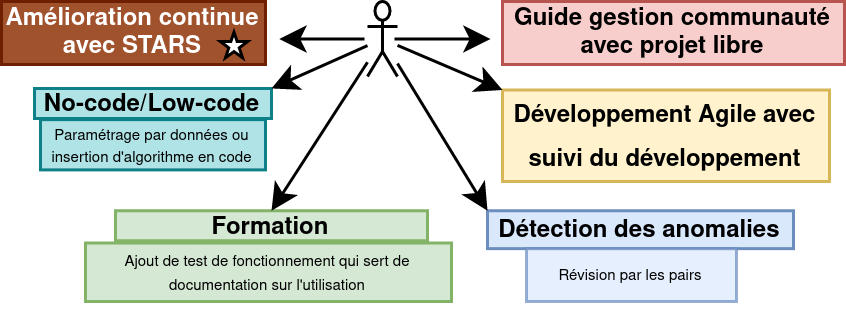
\includegraphics[width=5in]{images/developpeur_outil_developpement.drawio.png}
\caption{Intéraction entre les développeurs et les outils de développement dans un réseau d'entraide}
\label{fig:dia_outil_dev_reseau_entraide}
\end{figure}

\subsection{Avancement de la technopoïèse}\label{avancement_technopoiese}
Voir Figure~\ref{fig:dia_auto_machine_discussion}, la réingénierie manuelle est le processus habituel d'un développeur. Avec ce projet, nous avons une autopoïèse fonctionnelle semi-automatique, avec intervention humaine, puis une allopoïèse complète avec intervention humaine, lorsque cette dernière est en dehors des techniques maîtrisées par le robot logiciel codeur.

Pour l'Allopoïèse, le robot logiciel codeur vient assister l'intervention humaine à $H_0$ et $H_1$, qui permet de passer des méta-données, sur le module désiré, à une nouvelle version de ce module. Après une modification, il faut boucler avec le mode direct et le mode indirect du générateur de code pour avoir une version stable.

Pour l'Autopoïèse, la génération de code se fait directement sur le module de génération de code, c'est-à-dire que la machine est mise à jour avec l'assistance de la machine. L'humain intervient dans l'adaptation de la fonctionnalité et la correction de technique d'ingénierie au moment de la génération, aux endroits $H_0$ et $H_1$. À la fin de la modification, il faut boucler avec le mode direct et le mode indirect du générateur de code pour avoir une version stable de soi-même. Puisque le générateur de code génère le générateur de code, il y a des techniques et guides d'utilisation qui sont mis à la disposition dans le projet pour éviter de s'auto-écraser\footnote{C'est un problème qui peut arriver fréquemment dans ce système, de perdre des modifications en bouclant dû à une mauvaise manipulation ou une mauvaise configuration. Il faut toujours \textit{comiter} le travail avant de démarrer la machine.} et perdre son travail.

\begin{figure}
\centering
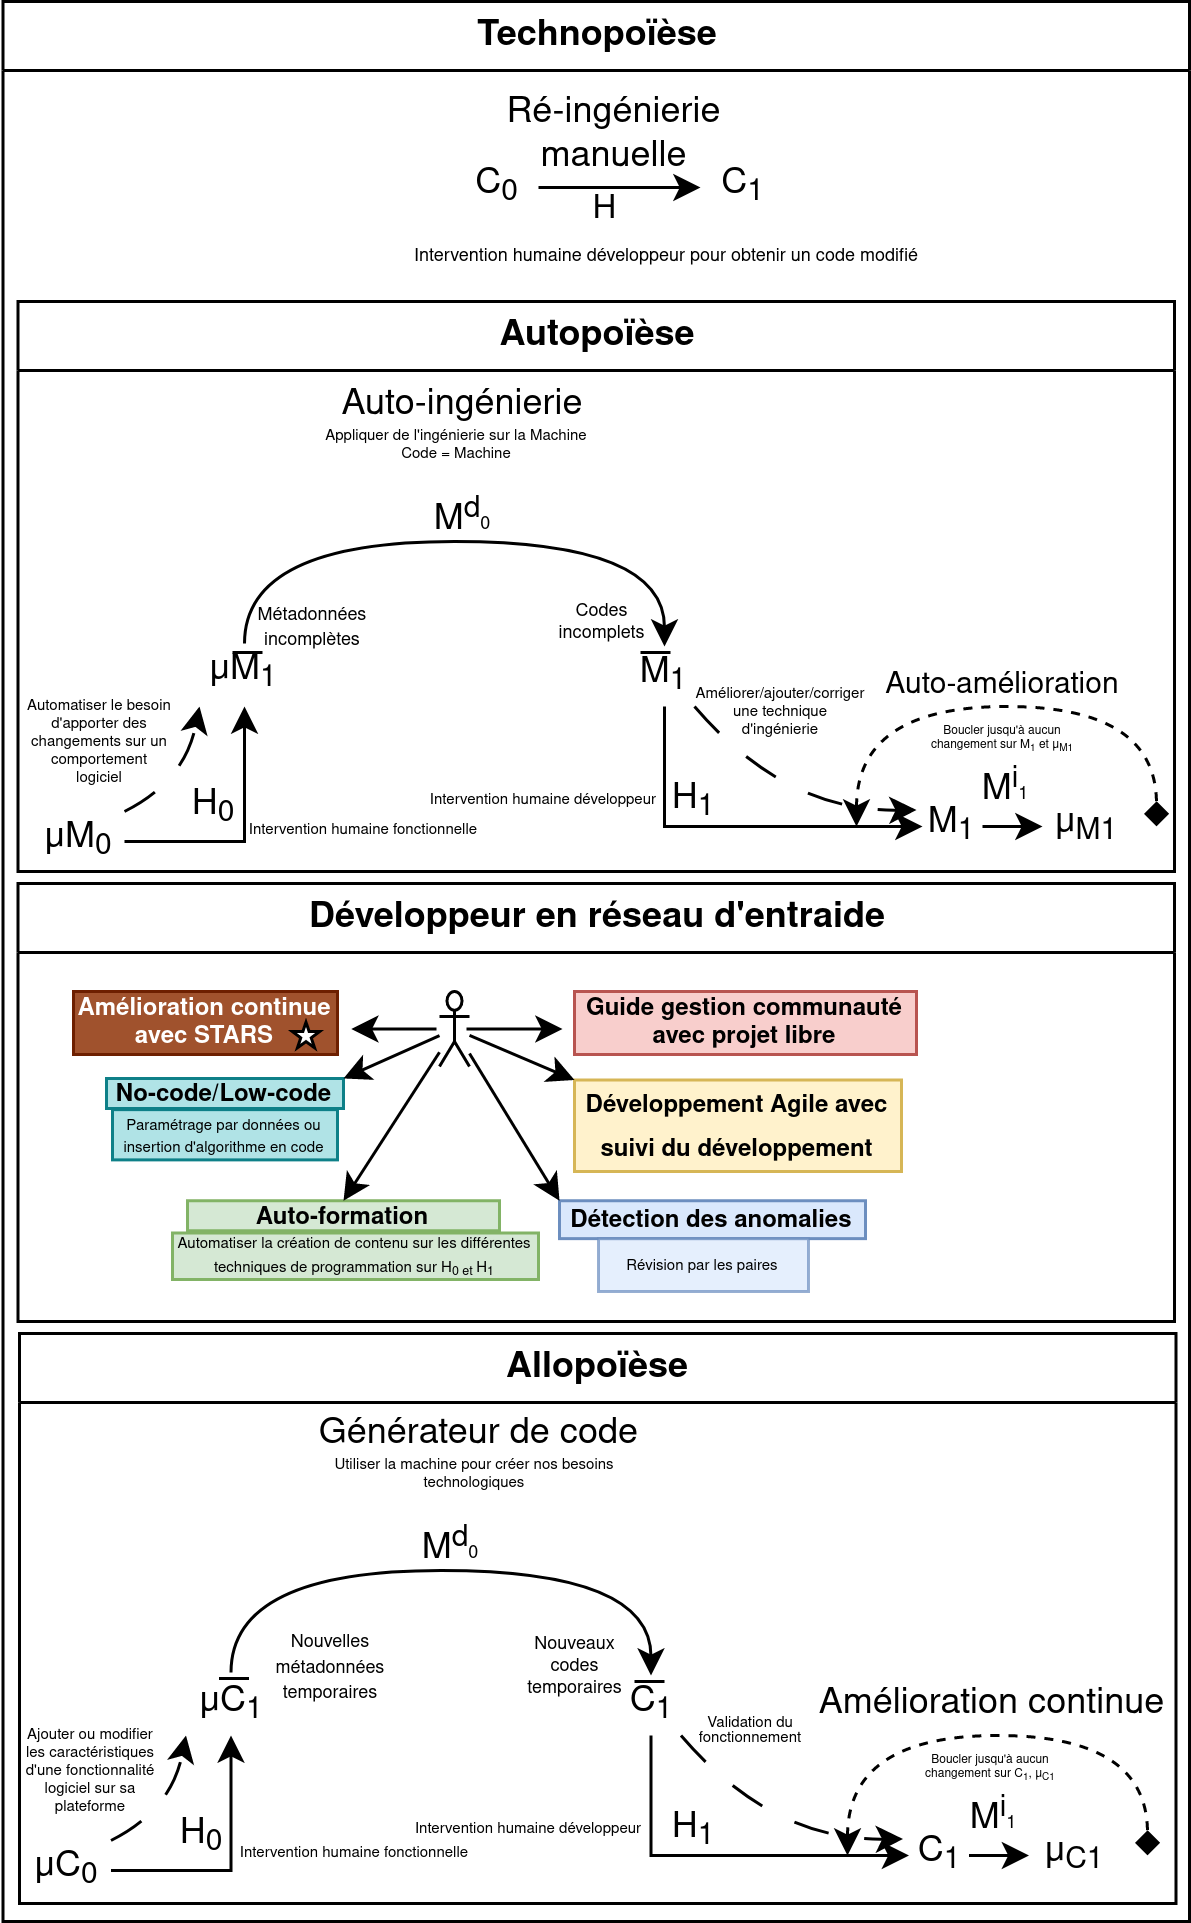
\includegraphics[height=8.5in]{images/auto_machine_discussion.drawio.png}
\caption{Architecture du générateur de code}
\label{fig:dia_auto_machine_discussion}
\end{figure}

\subsection{Réalisation du robot logiciel générateur de code}
Dans la revue littérature section~\ref{robot_logiciel_developpeur_revue}, nous avons déterminé 4 critères pour définir un robot logiciel codeur :

\subsubsection{Autonomie}
Nous avons des résultats qui démontrent 100\% d'autonomie dans quelques contextes, voir les résultats sur les tests de validation Section~\ref{test_validation_generation_code_resultat}. Cependant, le robot logiciel codeur n'est pas 100\% autonome pour tous les contextes, il a besoin d'intervention humaine pour des personnalisations ou des techniques non supportées, voir Section~\ref{avancement_technopoiese}.

% TODO une fois qu'on aura supporté plus de technique et l'autopoïèse entière, la prochaine étape serait de le faire fonctionner en continue. Bien qu'il soit capable via l'interface graphique, les efforts n'ont pas été effectué pour cette capacité.

\subsubsection{Adaptable}
Le robot logiciel codeur est adaptable, il génère 6 composantes, voir résultat d'architecture section~\ref{architecture_result} : web, \textit{website}, portail, \textit{snippet}, migration de données entrantes et migration de modèle de données entrantes. De plus, il est capable d'interagir avec des technologies en dehors d'Odoo comme extraire du code externe en PHP du logiciel SuiteCRM et des bases de données externes (MySQL/SQL Server/PostgreSQL) pour importer des modèles de données et migrer des données.

% TODO il faudrait supporter la génération de technologies externes, nous travaillons présentement à générer des applications mobiles natives, ou même générer des modules sur d'autres plateforme ERP tel que Tryton ou NextERP.

\subsubsection{Compétences techniques}
Le robot logiciel codeur contient plusieurs compétences techniques qui sont décrites dans les résultats section~\ref{result_technique_developpe}. De plus, il permet la personnalisation pour chacune des composantes du nombre de champs, des types de champs et du type d'affichage associé aux champs.

% TODO les techniques ont été développés comme preuve de concept, il manque de mâturité et de personnalisation. 

\subsubsection{Compétences sociales}
Le robot logiciel codeur donne accès à des outils pour le développeur. Il y a une interface graphique LCNC qui permet la paramétrisation pour la génération de code. Il y a aussi une interface de code pour paramétrer le fonctionnement de la génération accompagnée de la rétro-ingénierie et il permet d'accompagner le développeur dans l'évolution de son module. Il contient aussi une fonctionnalité pour afficher les différences de code entre la version précédente et la version générée, il permet de créer des statistiques sur les lignes de codes et il permet de montrer la couverture de code.

% TODO manque l'outil en temps réel, ce n'est pas supporté dans Odoo, il faut utiliser une application tierce tel que Etherpad et ajouter les méthodes de synchronisation des mises à jour sur les données. Il manque l'accès directe aux script à la racine du projet ERPLibre pour contrôler les outils de contrôle de la qualité. Collaboration, conscience professionnelle, résolutions de problèmes en équipe, communication efficace, adaptivité sur les livrables et exigences clientes

% \subsection{DevOps}
% Il faudrait mettre en place les outils de dev ops.
% Mise à jour des bibliothèques (avoir une vue d’ensemble autre que Poetry)

% \subsection{Gestion de communauté}
% Un downtime de plus d’une journée cause drastiquement un abandon des participants à l’utilisation d’une technologie au sein d’une autre.

% \subsection{Réseau d’entraide}

% Il doit y avoir un responsable pour chaque localité accompagné du robot logiciel codeur pour répondre à ses besoins de numérisations via une souveraineté numérique. C’est le gestionnaire de communauté.

% Chaque projet d’urgence doit être capable d’avoir une équipe en charge pour accélérer la résolution de problèmes locaux.

% \subsection{Technopoïèse}
% À titre de discussion sur la signification de technopoïèse.

% Auto-répliqueur : une machine qui se copie lui même.
% Allopoïèse : une machine qui crée une autre machine avec des éléments extérieurs, l’inverse de l’autopoïèse.
% Autopoïèse : la propriété d’un système de se produire lui-même, en permanence et en intéraction avec son environnement, et ainsi de maintenir son organisation (structure) malgré son changement de composants (matériaux) et d’informations (données).
% REF https://fr.wikipedia.org/wiki/Autopo%C3%AF%C3%A8se
% Technopoïèse : une technologie qui a la propriété de se produire lui-même …
% «Une technologie pour étudier la vie humaine, des nouvelles sociétés et les accompagner dans leur développement d’autopoïèse. »
% La technopoïèse doit être développée dans un contexte de logiciel libre pour mettre au centre le réseau d’entraide et avoir le contrôle sur les dérives non éthiques.
% Outil passif utilisé par les humains pour jouer un rôle actif dans la création de la société et de la culture en façonnant leur environnement et leur mode de vie. Comprendre comment les technologies influencent la façon dont les individus interagissent et comment elles peuvent être utilisées pour améliorer la vie des gens, de manière responsable et éthique.

% \subsection{robot logiciel codeur libre}

% Les robots codeurs peuvent être programmés pour effectuer différentes tâches, telles que la génération de code source, la correction de bugs, l'optimisation des performances, la maintenance des systèmes et la gestion de versions. Certains robots codeurs peuvent même apprendre à partir d'exemples de code existant et développer des algorithmes en se basant sur des données d'entrée.

% Les robots codeurs peuvent également améliorer la qualité du code en réduisant les erreurs humaines, en accélérant les tests et en appliquant des pratiques de codage cohérentes.»

% TODO projet d’impression 3D à distance, avec des propriétaires de machines qui les entretiennent.

% TODO connaissance de la physique et les appliquer, optimisation pour accompagner les communautés dans leur gestion d’urgence
% TODO doit reproduire les 4 libertés pour l’utilisation, l’accompagner dans son développement pour améliorer ses habitudes de vies par lui même sans dépendre d’autrui, restons en communauté locale pour réduire la consommation.
% TODO faciliter l’intégration de l’intération entre notre robot personnel et celui d’une technologie externe.

